\documentclass[12pt]{article}

\usepackage{pdfpages}
\usepackage[utf8]{inputenc}
\usepackage{amsmath}
\usepackage{amssymb}
\usepackage{algorithm}
\usepackage{tikz}
\usetikzlibrary{automata,positioning}

\usepackage{algpseudocode}
\algnewcommand{\LineComment}[1]{\State \(\triangleright\) #1}
\usepackage{fancyhdr}
\pagestyle{fancy}
\renewcommand\headrule{}
\fancyhead[L]{Gregor Bankhamer 1220843 Wolfgang Kremser 1222223 Wang Michelle Yih-chyan 1641792}
\newcommand{\RN}[1]{%
  \textup{\uppercase\expandafter{\romannumeral#1}}%
}

\DeclareMathOperator{\ggT}{ggT}


\setlength\parindent{0pt}

\begin{document}

\section *{Exercise 4}
In agnostic PAC Learning D is the distribution over $X$ x $Y$. Assuming the Realizability of $H$, Y relies only on X. Therefore, the Distribution $D$ relies only on X.
$L_D \leq min_h \in H L_D (h) + \epsilon$.
\\ \\
There exist a super function $f \in H$ and $L_D (f) = 0$ such that
$min_{h \in H} L_D (h)+L_D (f) = 0$; therefore
$L_D(h) \in 0+ \epsilon = \epsilon$

\section*{Exercise 5}

Under the assumption of realizability, the error we can make is bound between the tightest circle that encloses all equally labeled samples and the circle which is just before the first differently labeled sample. The annulus of these circles is colored red in the figure. Somewhere on that annulus lies the circle which represents the true labeling function $f$.
\\ \\
Let $f$ have radius $r_f$. We chose a circle $h$ which represents a hypothesis with the smallest radius $r_h$ such that $P(r_h \leq ||x|| \leq r_f) < \epsilon$. Now, let A be all radii between $r_h$ and $r_s$, i.e $A := \{x : r_h \leq ||x|| \leq r_s\}$. By definition of $r_h$, $P(x \in A) \geq \epsilon$.
\\ \\
Therefore, the chance to not make an error greater than $\epsilon$ is $P(x \notin A) \le (1 - \epsilon)$. For $m$ samples we have the chance of $(1-\epsilon)^m \leq e^{-m\epsilon} \geq \delta$, leading to $m \geq \frac{1}{\epsilon} log(\frac{1}{\delta})$


\begin{figure}
	\centering
	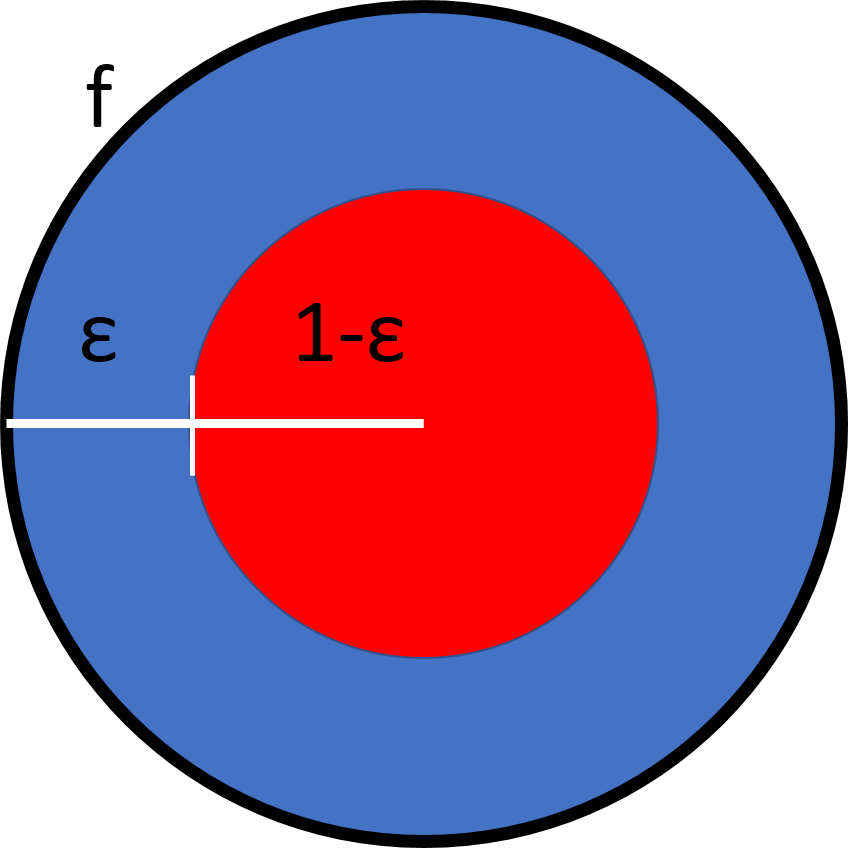
\includegraphics[width=0.7\linewidth]{Bild1}
\end{figure}



\end{document}
